\section{Existing Solutions Sufficient?}
\label{sec:existing}
In this section, we explore the third question: are existing network-layer solutions sufficient to meet the requirements imposed by the applications in \dis? We start by describing the methodology (\S\ref{ssec:ssmethod}), and then evaluate the network-level (\S\ref{ssec:nlp}) and application-level performance (\S\ref{ssec:alp}) in \dis using existing network-level solutions.

\subsection{Methodology}
\label{ssec:ssmethod}
We explore the sufficiency of existing network-layer solutions for \dis in two steps. First, we take the flows generated from \S\ref{sec:workloads} and simulate the network-layer performance (flow completion time) for these flows. We then return to our emulator, take the respective flow completion time for flows, and inject the respective latencies using SIT, as described in \S\ref{sec:requirements}, thus allowing us to evaluate the application level performance. 

For all the simulations in this section, we use the setup from \cite{phost}. In particular, we simulate a $144$-node full bisection bandwidth fat-tree topology with $40$Gbps access link capacity. \rc{What else do we need to describe?} However, there are multiple challenges in executing the above two steps that we had to resolve.

\paragraphb{Scaling up}

\paragraphb{Latency injection for long flows}

\paragraphb{Level of disaggregation: $3\times$ problem?}

\subsection{Network-level performance}
\label{ssec:nlp}

%
\begin{figure}
  \centering
    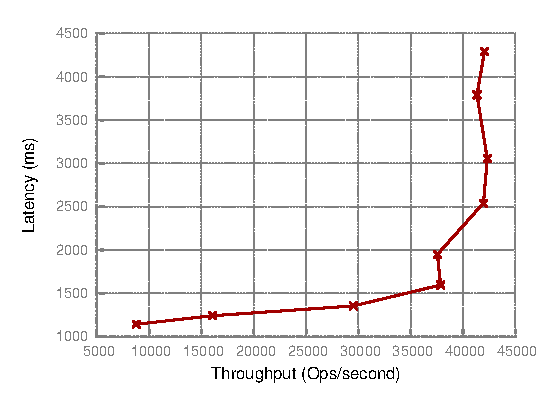
\includegraphics[width = 2.5in]{img/thvsla_get} 
  \caption{\small{\rqc{The mean slowdown for pFabric/pHost for each of the six applications. Perhaps, we should show results across bins of flow sizes.}}}
  \label{fig:phostp}
\end{figure}
%

\subsection{Application-level performance}
\label{ssec:alp}

%
\begin{figure}
  \centering
    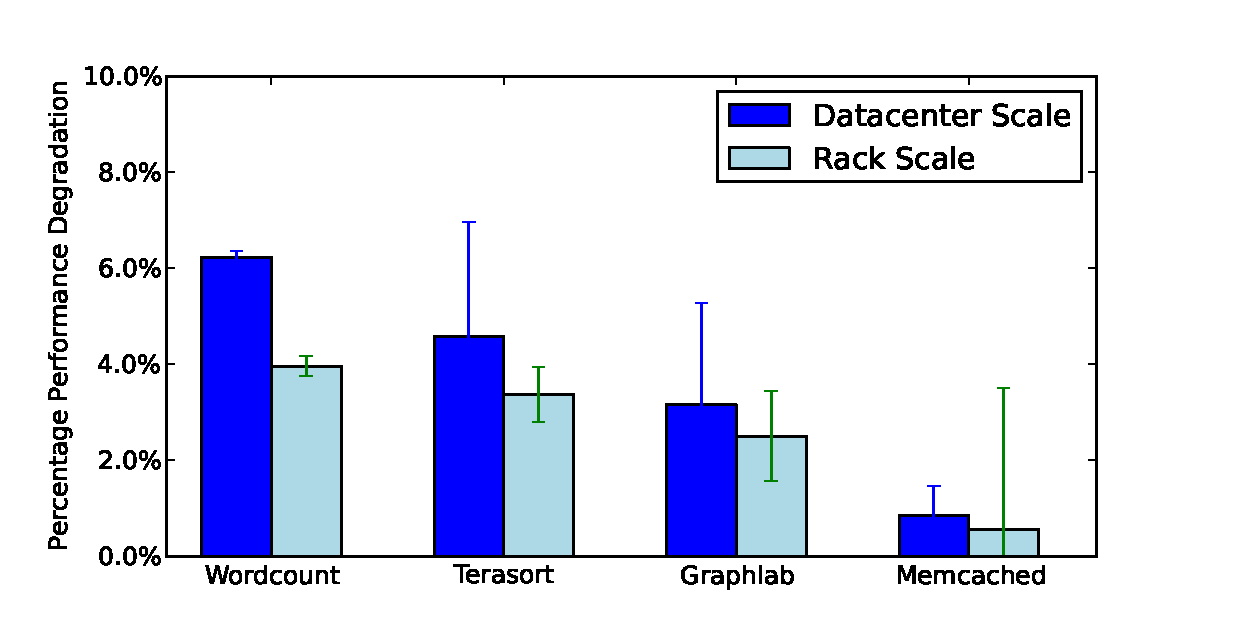
\includegraphics[width = 2.5in]{img/slowdown.eps} 
  \caption{\small{\rqc{Application layer slowdown for each of the six applications.}}}
  \label{fig:appfabric}
\end{figure}
%
